\documentclass[10pt,twocolumn,a4paper]{article}
\usepackage[margin=0.62in,columnsep=0.24in,top=0.7in,bottom=0.75in]{geometry}
\usepackage{fontspec}
\setmainfont{TeX Gyre Termes}
\setsansfont{TeX Gyre Heros}
\setmonofont{DejaVu Sans Mono}[Scale=0.8]
\usepackage[dvipsnames]{xcolor}
\definecolor{ieeeblue}{HTML}{0072BC}
\usepackage{titlesec}
\usepackage{booktabs}
\usepackage{array}
\usepackage{amsmath}
\usepackage{caption}
\usepackage{enumitem}
\usepackage{fancyhdr}
\usepackage{graphicx}
\graphicspath{{../../figs/}}
\usepackage{tikz}
\usetikzlibrary{positioning,arrows.meta,shapes.geometric}
\usepackage[hidelinks]{hyperref}

\titleformat{\section}{\sffamily\bfseries\small\color{ieeeblue}}{\thesection.}{0.5em}{\MakeUppercase}
\titleformat{\subsection}{\sffamily\bfseries\footnotesize\itshape}{\thesubsection.}{0.5em}{\MakeUppercase}
\titleformat{\subsubsection}{\sffamily\footnotesize}{\arabic{subsubsection})}{0.5em}{\MakeUppercase}
\titlespacing*{\section}{0pt}{9pt}{4pt}
\titlespacing*{\subsection}{0pt}{7pt}{3pt}
\renewcommand{\thesection}{\Roman{section}}
\renewcommand{\thesubsection}{\Alph{subsection}}
\makeatletter\renewcommand{\p@subsection}{\thesection-}\makeatother

\captionsetup[table]{font=footnotesize,labelfont={sf,bf,color=ieeeblue},labelsep=period,justification=raggedright,singlelinecheck=false,skip=3pt}
\captionsetup[figure]{font=footnotesize,labelfont={sf,bf,color=ieeeblue},labelsep=period,justification=raggedright,singlelinecheck=false}

\pagestyle{fancy}\fancyhf{}
\renewcommand{\headrulewidth}{0.4pt}
\fancyhead[L]{\footnotesize\sffamily M. Balaji \textit{et al.}: Network-Level Evaluation of IoMT Intrusion Detection}
\fancyfoot[C]{\footnotesize\sffamily\thepage}
\setlength{\parindent}{1.1em}
\setlength{\tabcolsep}{2.9pt}
\renewcommand{\arraystretch}{1.1}
\newcommand{\pending}[1]{\textcolor{red}{\textbf{[PENDING: #1]}}}

\begin{document}
\twocolumn[
\begin{@twocolumnfalse}
\vspace{-6pt}
{\footnotesize\sffamily\itshape Review 3 manuscript, October 2026. Code, raw simulation logs and analysis scripts accompany this manuscript (Section~\ref{sec:repro}).}
\vspace{4pt}\hrule height 0.4pt
\vspace{10pt}

{\sffamily\bfseries\fontsize{20}{24}\selectfont\color{ieeeblue}
Detection Rate Is Not Enough: A Simulation-in-the-Loop\\ Framework for Network-Level Evaluation of\\ IoMT Intrusion Detection\par}
\vspace{9pt}
{\sffamily\bfseries\fontsize{10.5}{13}\selectfont MALIKA BALAJI, NEHAA PRABHU, ROHITH PRANOV, SANHIT MUTHUSWAMY, AND RAKSHAN V. P.\par}
\vspace{2pt}
{\footnotesize School of Computer Science and Engineering, Vellore Institute of Technology, Vellore 632014, India}
\vspace{10pt}

\noindent\begin{minipage}{\textwidth}
\footnotesize
\textbf{\color{ieeeblue}ABSTRACT}\quad
Dataset-based evaluation cannot expose network-level failure modes. Intrusion detection systems for the Internet of Medical Things (IoMT) are trained and scored on stored captures, where a detector has no queue to slow down, no legitimate device to disconnect, and no feedback from its own decisions. We present a five-step methodology for placing a published IoMT intrusion detector inside a network simulator: obtain the system, audit its reported numbers arithmetically, rebuild it under leakage controls, place its decision rule in the data path of an ns-3 fog network, and evaluate it across 20 seeds, a scenario matrix, a sensitivity analysis and measured inference costs. Applying it to a recent fog-based system and two further IoMT detectors from 2025 and 2026 shows the following. Re-derivation from published confusion matrices confirms a positive-class inversion and transposed precision and recall in one paper and a train/test split drawn after oversampling in two of three; in one of them the test set holds more attack records than the whole dataset. On a public IoMT dataset, oversampling before the split alone raises F1 from 0.673 to 0.959 over 20 partitions, and duplicate rates depend on the feature space retained, from 0.52\,\% of raw rows to 98.95\,\% of modelling vectors on Edge-IIoTset. In the network, three threshold rules block every attacker in the baseline yet quarantine between 45\,\% and 100\,\% of legitimate wearables, and the published flat rule quarantines all of them in every one of 16 scenarios. A congestion-coupled threshold latches off under load in 20 of 20 baseline seeds and in 11 of 15 further scenarios at the same cost; it also fails at an otherwise safe cost when one fog node carries the flood, and on a Raspberry Pi 4 running the trained ensemble it latches at the Review~2 attack scale even at the board's idle inference cost (3.0\,ms per window). Three mitigations each restore full detection in every run, but on the Pi wearable telemetry still waits 0.3 to 1.2\,s behind each flood. A trade-off analysis shows that threshold adaptation slides along a curve set by the information it acts on, while gating it with a flow classifier of low false-positive rate moves the curve, cutting false alerts by a third with no missed attacker. We also report that a three-branch ensemble does not beat its best branch, that attack types withheld from training go almost undetected, and that the requested cross-dataset transfer is infeasible because the two datasets share no features. Code, raw runs and analysis are released.

\vspace{6pt}

\textbf{\color{ieeeblue}INDEX TERMS}\quad Internet of Medical Things, intrusion detection, evaluation methodology, network simulation, ns-3, data leakage, adaptive thresholds, explainable AI, reproducibility.
\end{minipage}
\vspace{14pt}
\end{@twocolumnfalse}
]

\section{Introduction}\label{sec:intro}
\noindent The Internet of Medical Things (IoMT) places networked sensors and actuators directly in the clinical care path. A compromised infusion pump or a silenced cardiac monitor is a patient-safety incident before it is an information-security incident, and this has produced a large body of work on intrusion detection systems (IDS) for IoMT and fog deployments \cite{berguiga2025,hosain2025,shaikh2024,ghourabi2025,alalhareth2024,lazrek2024,sogut2026}.

Almost all of that work is evaluated the same way. A public capture is obtained, class imbalance is corrected, a classifier is trained, and accuracy, precision, recall and F1-score are reported, now routinely above 99\,\% \cite{berguiga2025,hosain2025,shaikh2024,sogut2026}. \textbf{Dataset-based evaluation cannot expose network-level failure modes.} A stored dataset has no queue, so the inference cost of a detector never becomes delay. It has no legitimate devices that can be quarantined, so a rule that disconnects every wearable on a ward scores the same as one that disconnects none, provided both catch the same attackers. And it has no feedback from the detector's decisions to the traffic it later observes, so any failure that lives in that loop is invisible by construction.

This paper presents a methodology for placing a published IoMT IDS inside a network simulator, together with an audit procedure for its reported numbers, and applies both to a recent fog-based system, HIDS-IoMT \cite{berguiga2025}. We chose that system because it is unusually explicit: it states its threshold ($\tau = 500$\,ms), its inspection period, its datasets and hardware, and it publishes the confusion matrices behind its headline metrics. Explicitness is what makes an audit possible, and we treat it as a virtue. To test whether what we find is specific to one paper, we apply the same audit to two further IoMT IDS published in 2025 and 2026 \cite{hosain2025,tarish2026}, and measure duplicate records and train/test leakage across four public datasets.

Our contributions are:
\begin{enumerate}[leftmargin=1.3em,itemsep=1pt,topsep=2pt]
\item \textbf{A reproducible audit methodology.} Five arithmetic checks that a reader can run on a published paper without its code or data (positive-class inversion, transposed precision and recall, partitioning after oversampling, unhandled duplicates, irreproducible metrics), applied to three IoMT IDS papers.
\item \textbf{A network simulation framework.} A five-step procedure and an open ns-3 implementation that places a detector's decision rule in the data path of a fog network, measures what dataset evaluation cannot (collateral quarantine of legitimate devices, delay including inspection queueing, control overhead, inspection energy), and evaluates it over 20 seeds, a one-factor-at-a-time scenario matrix, a sensitivity analysis and measured inference costs.
\item \textbf{Empirical findings, including negative results.} In the baseline, detection rate is identical across three threshold architectures while collateral quarantine ranges from 45\,\% to 100\,\% of the wearable estate, and the published flat rule quarantines every wearable in all 16 scenarios; a congestion-coupled threshold latches off in 20 of 20 baseline seeds under load and in 11 of 15 further scenarios at the same cost, and three mitigations each restore full detection in every run; threshold adaptation alone moves operating points along a fixed trade-off curve, while gating it with a flow classifier moves the curve; oversampling before partitioning inflates F1 from 0.673 to 0.959 on an IoMT dataset; and duplicate rates depend on the feature space, from 0.52\,\% of raw rows to 98.95\,\% of modelling vectors on Edge-IIoTset. We also report that our deep ensemble does not beat its best branch, that one explanation method is unstable, and that the detector does not recognise attack types withheld from training.
\end{enumerate}

Section~\ref{sec:related} positions the work. Section~\ref{sec:framework} formalises the framework, and Section~\ref{sec:setup} describes how it was applied. Section~\ref{sec:results} reports results, and Sections~\ref{sec:discussion} to \ref{sec:conclusion} discuss, bound and conclude.

\section{Related Work}\label{sec:related}

\subsection{IoMT intrusion detection}
\noindent Recent IoMT detectors span convolutional and recurrent hybrids \cite{berguiga2025,shaikh2024}, gradient-boosted trees with post-hoc explanation \cite{hosain2025}, federated training across clinical sites \cite{ghourabi2025}, meta-learned ensembles \cite{alalhareth2024}, feature-selection pipelines \cite{lazrek2024}, lightweight attention networks \cite{sogut2026} and CNN classifiers on the CICIoMT2024 benchmark \cite{mohammadi2024,dadkhah2024}. They are evaluated on public captures, principally WUSTL-EHMS-2020 \cite{wustl}, IoTID20 \cite{ullah2020}, Edge-IIoTset \cite{ferrag2022} and CICIoMT2024 \cite{dadkhah2024}, and they report accuracy at or above 97\,\%, most above 99\,\%. HIDS-IoMT \cite{berguiga2025} adds fog deployment on a Raspberry Pi and is the only one of these to state a decision threshold and an inspection period, which is why it is the object of our network-level study. Its prior-work neighbour in our own laboratory, a stacking ensemble on CICIDS2017 \cite{badiyani2026}, applies its balancing step before the train/test split, the same ordering we examine in Section~\ref{sec:audit}. When most of a literature reports figures within a point of the ceiling, the interesting question becomes whether the evaluation instrument still resolves anything.

\subsection{Evaluation pitfalls and dataset flaws}
\noindent Arp \textit{et al.} \cite{arp2022} catalogue pitfalls in learning-based security, including data snooping and inappropriate baselines, and show them to be common in top-venue work. For network IDS specifically, Engelen \textit{et al.} \cite{engelen2021} and Lanvin \textit{et al.} \cite{lanvin2023} document generation, flow-construction and labelling errors in CICIDS2017 that change benchmark conclusions, Liu \textit{et al.} \cite{liu2022} extend this to CSE-CIC-IDS2018, and Flood \textit{et al.} \cite{flood2024} define measurable ``design smells'' across seven benchmarks. Galal \cite{galal2026}, concurrently with our project's own finding, reports that missing values in Edge-IIoTset are serialised differently in normal and attack files and leak the label.

Bouke and Abdullah \cite{bouke2023} study how pattern leakage introduced during preprocessing affects the reliability of machine-learning IDS on benchmark datasets. Our work starts from that concern and extends it in three directions. First, we treat exact duplicate records as a leakage vector that survives a correct split order and show that its size is a property of the feature space a pipeline keeps, not of the file. Second, we audit published confusion matrices arithmetically, which exposes partitions drawn from an oversampled population without any access to code. Third, we move evaluation from the dataset to the network, where failure modes such as false quarantine of legitimate devices and a latch-off of congestion-coupled thresholds appear that no dataset can show.

\subsection{Network simulation for detector evaluation}
\noindent Simulation is used to evaluate detectors in other domains: Meyer \textit{et al.} \cite{meyer2024} build an OMNeT++ toolchain that injects anomalies into time-sensitive automotive networks and show that detection quality depends on the traffic mix. In IoT security, ns-3 is mostly used to generate data for offline classifiers \cite{chaudhari2023} or to measure the impact of attacks on network performance \cite{rajab2025}, and recent testbeds emulate mixed traffic for live detection \cite{rustam2025}. We found no IoMT work that places a published detector's decision rule in the forwarding path and measures what it does to legitimate devices; that is the gap this paper addresses.

\subsection{Adaptive thresholds}
\noindent Dynamic thresholds that follow recent error statistics are well established in anomaly detection \cite{hundman2018,yuan2024,ding2026}. They adapt to the detector's own error distribution. The congestion-coupled rule we study instead adapts to the network's queue state, and Section~\ref{sec:latch} shows why that coupling is dangerous when the detector sits in the data path.

\section{A Framework for Network-Level IoMT IDS Evaluation}\label{sec:framework}
\noindent The framework has five steps (Fig.~\ref{fig:framework}). Each produces an artefact that the next consumes, and each has an explicit failure condition, so a step that cannot be completed is reported as such rather than worked around.

\begin{figure}[t]
\centering
\resizebox{\columnwidth}{!}{%
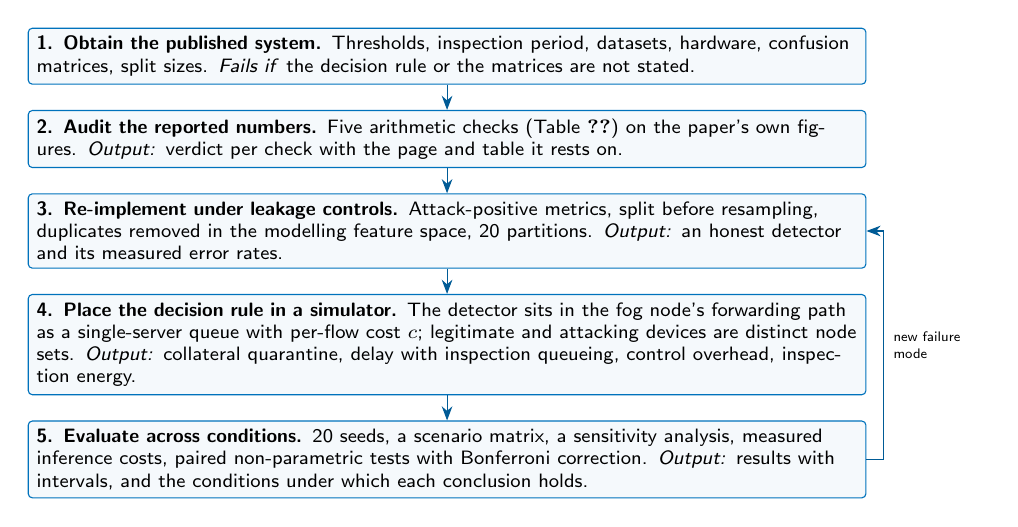
\begin{tikzpicture}[node distance=3.2mm, every node/.style={font=\scriptsize\sffamily},
  box/.style={draw=ieeeblue, rounded corners=1.5pt, align=left, text width=0.86\columnwidth, inner sep=3pt, fill=ieeeblue!4},
  arr/.style={-{Stealth[length=1.8mm]}, draw=ieeeblue!80!black}]
\node[box] (s1) {\textbf{1. Obtain the published system.} Thresholds, inspection period, datasets, hardware, confusion matrices, split sizes. \emph{Fails if} the decision rule or the matrices are not stated.};
\node[box, below=of s1] (s2) {\textbf{2. Audit the reported numbers.} Five arithmetic checks (Table~\ref{tab:checks}) on the paper's own figures. \emph{Output:} verdict per check with the page and table it rests on.};
\node[box, below=of s2] (s3) {\textbf{3. Re-implement under leakage controls.} Attack-positive metrics, split before resampling, duplicates removed in the modelling feature space, 20 partitions. \emph{Output:} an honest detector and its measured error rates.};
\node[box, below=of s3] (s4) {\textbf{4. Place the decision rule in a simulator.} The detector sits in the fog node's forwarding path as a single-server queue with per-flow cost $c$; legitimate and attacking devices are distinct node sets. \emph{Output:} collateral quarantine, delay with inspection queueing, control overhead, inspection energy.};
\node[box, below=of s4] (s5) {\textbf{5. Evaluate across conditions.} 20 seeds, a scenario matrix, a sensitivity analysis, measured inference costs, paired non-parametric tests with Bonferroni correction. \emph{Output:} results with intervals, and the conditions under which each conclusion holds.};
\draw[arr] (s1) -- (s2); \draw[arr] (s2) -- (s3); \draw[arr] (s3) -- (s4); \draw[arr] (s4) -- (s5);
\draw[arr] (s5.east) -- ++(2.2mm,0) |- node[pos=0.25, right, align=left, font=\tiny\sffamily, text width=1.1cm]{new failure mode} (s3.east);
\end{tikzpicture}}
\caption{The five-step framework. The feedback arrow is how mitigations enter: a failure found in step 5 is fixed in the rule and re-evaluated, as for the latch-off in Section~\ref{sec:latch}.}
\label{fig:framework}
\end{figure}

\subsection{Step 2: the audit checks}
\noindent The checks need only quantities a paper prints (Table~\ref{tab:checks}). Check (a) recomputes precision and recall from the confusion matrix with each class as positive and asks which convention reproduces the printed figures. Check (b) asks whether the printed precision equals the recomputed recall and vice versa, or whether the printed formulae are swapped. Check (c) sums the reported split sizes and compares them with the dataset sizes before and after oversampling; a test fold that matches the oversampled total, or that contains more minority samples than the raw data holds, proves the partition was drawn after oversampling. Check (d) searches the text for duplicate handling and, where the data is available, measures duplicates directly. Check (e) records any printed metric that cannot be reproduced from the matrix.

\begin{table}[t]
\caption{Audit checks. Each needs only the paper's printed numbers.}
\label{tab:checks}
\centering\footnotesize
\begin{tabular}{@{}p{0.07\columnwidth}p{0.36\columnwidth}p{0.5\columnwidth}@{}}
\toprule
& \textbf{Check} & \textbf{Evidence that confirms it} \\
\midrule
a & Positive-class inversion & printed P/R reproduce only with Normal as positive \\
b & Transposed precision/recall & printed P equals recomputed R, or formulae swapped \\
c & Partition after oversampling & split sizes sum to the oversampled total; test minority exceeds raw minority \\
d & Duplicates unhandled & no mention, and duplicates present in the data \\
e & Irreproducible metric & a printed value not derivable from the matrix \\
\bottomrule
\end{tabular}
\end{table}

\subsection{Step 4: the detector in the data path}
\noindent A fog node with per-flow inspection cost $c$ serves at most $S = 1/c$ flows per second. Its queue occupancy $L \in [0,1]$ (queue length over capacity) is the load signal an adaptive rule may read. Each inspected flow updates a per-source record of inter-arrival gaps, and a source accumulating $p$ violations of the rule (the \emph{patience}) is quarantined: its later packets are dropped at the fog node and a quarantine notice is sent to the controller and to every peer fog node. A quarantined legitimate device is a false positive at the network level, and it is counted separately from false-positive alerts.

Two measurements matter that a flow monitor on the wire does not provide. The first is application-level delay: each packet carries its send time, and delay is measured when the fog node finishes inspecting it, so inspection queueing is included. The second is inspection energy, $E = N P_{\mathrm{idle}} T + (P_{\mathrm{active}} - P_{\mathrm{idle}})\, n_{\mathrm{insp}}\, c$ for $N$ fog nodes over $T$ seconds and $n_{\mathrm{insp}}$ inspections. The power figures are model parameters (6.4\,W active, 2.7\,W idle, a nominal fog-node envelope) until replaced by a meter reading (Section~\ref{sec:hardware}); we therefore compare energy only between rules under identical parameters.

\subsection{Step 5: statistical protocol}
\noindent Every configuration is run with independent ns-3 run numbers $1, \dots, n$ (seed 42), with $n = 20$ for the baseline and $n$ stated for every other experiment, varying sender start offsets and telemetry jitter. Rules compared at the same run number see identical traffic, so comparisons are paired: we use the Wilcoxon signed-rank test and correct with Bonferroni across each family of tests, and report means with standard deviations and 95\,\% confidence intervals ($t$ distribution, $n-1$ degrees of freedom). Every raw run is stored as one line of key-value output before aggregation, so every number in this paper can be re-derived from the logs.

\subsection{Reuse}
\noindent Nothing in steps 1 to 5 is specific to HIDS-IoMT. Another detector enters by supplying its decision rule (a function from per-source state and node load to a violation) and its per-flow cost; another dataset enters through steps 2 and 3 unchanged. The simulator, runner and analysis scripts are released (Section~\ref{sec:repro}).

\section{Applying the Framework}\label{sec:setup}

\subsection{Systems audited}
\noindent HIDS-IoMT \cite{berguiga2025} is the primary subject. For the broadened audit we screened ten open-access IoMT IDS papers from 2024 to 2026 and retained the two whose confusion matrices are given as numbers rather than images, with metrics for the same experiment: XAI-XGBoost \cite{hosain2025} and a leakage-free Nyström sampling study \cite{tarish2026}, both evaluated on WUSTL-EHMS-2020.

\subsection{Datasets}
\noindent IoTID20 \cite{ullah2020} (625,783 flow records, CICFlowMeter features), Edge-IIoTset \cite{ferrag2022} (the 157,800-row file released for machine learning, per-packet tshark fields), WUSTL-EHMS-2020 \cite{wustl} (16,318 records, Argus flow features plus eight biometric fields) and, for duplicate measurement only, the Friday DDoS day of CICIDS2017 \cite{sharafaldin2018}. IoTID20 figures in this paper come from the project's own pipeline run; the other three were measured for this revision from mirrored copies whose row and class counts match the published descriptions.

\subsection{Threshold architectures}
\noindent All rules decide the same question for each inspected flow: is this source's inter-message gap too short?
\begin{itemize}[leftmargin=1.2em,itemsep=1pt,topsep=2pt]
\item \textbf{A, flat} (the base paper): violation if the gap is below $\tau_0 = 500$\,ms, for every device.
\item \textbf{B, congestion-coupled EWMA}: violation if the source's EWMA gap ($\alpha = 0.3$) is below $\tau_0(1-L)$, so detection loosens as the fog queue fills. This is our reconstruction of a congestion-adaptive rule, not any published code.
\item \textbf{C, criticality-weighted} (our proposal): violation if the gap is below $\mathrm{clamp}(\tau_0\, w_d\, (1 + 0.3(L-0.5)), 50, 2000)$\,ms with device-class weights $w_d \in \{0.6, 0.8, 1.0, 1.3\}$ from life-critical to non-clinical.
\item \textbf{B$'$, mitigated B} (Section~\ref{sec:latch}): B with a hysteresis floor, a dual fixed threshold, or a capacity-coupled threshold.
\end{itemize}
Every rule quarantines a source after $p = 3$ violations unless stated.

\subsection{Network scenarios}
\noindent The baseline is the Review~2 scenario: 20 legitimate wearables (600\,ms telemetry, $\pm$40\,\% jitter), 60 attacker-bots (5\,ms flood), 4 fog nodes, star topology over 10\,Mb/s access and 100\,Mb/s backhaul links, 30 simulated seconds, per-flow inspection cost 500\,µs, balanced device mix. The scenario matrix varies one factor at a time from this baseline: wearables $\{10, 20, 40, 80\}$, attacker-bots $\{20, 40, 60, 80, 120\}$, fog nodes $\{1, 2, 4, 8\}$, topology (star, clustered wards with half the bots in one ward, a 4$\times$4 switch grid, a random geometric switch graph) and device mix (balanced, ICU-heavy 50/30/15/5\,\%, periphery-heavy 5/15/30/50\,\%), each at 500\,µs and at 2,000\,µs per flow. The full factorial would need 960 scenarios per architecture and inspection cost; we run the 16 one-factor scenarios and state the interaction we test separately (inspection cost against attack scale, Section~\ref{sec:latch}).

\subsection{Simulator validity}
\noindent The Review~3 simulator extends the Review~2 program. With every new option at its default it is the same program, and on the same ns-3 \cite{nsnam} build both produce identical detection counts (checked for all three rules at run 1). Moving the unmodified Review~2 program from the ns-3 build used in Review~2 to ns-3.44 changed its single-seed head-to-head counts (Table~\ref{tab:version}): architecture B went from 8 to 10 quarantined wearables and C from 9 to 10. Nothing in the model changed; the random stream mapping did. This is the strongest argument we have for the multi-seed protocol, and every network-level result below is a 20-seed distribution.

\begin{table}[t]
\caption{The same Review 2 program, run number 1, on two ns-3 builds. Single-seed results are not stable across simulator versions.}
\label{tab:version}
\centering\footnotesize
\begin{tabular}{@{}lccc@{}}
\toprule
\textbf{ns-3 build} & \textbf{A} & \textbf{B} & \textbf{C} \\
\midrule
Review 2 build & 327 / 60 / 20 & 303 / 36 / 8 & 296 / 29 / 9 \\
ns-3.44 & 321 / 60 / 20 & 300 / 39 / 10 & 291 / 30 / 10 \\
\bottomrule
\multicolumn{4}{@{}l}{\scriptsize Cells: alerts / false-positive alerts / wearables quarantined.}
\end{tabular}
\end{table}

\section{Results}\label{sec:results}

\subsection{Audit of reported metrics}\label{sec:audit}
\subsubsection{HIDS-IoMT}
Section III-G-4 of \cite{berguiga2025} states that SMOTE balancing yields 2,727,996 Edge-IIoTset instances, and its binary split (2,182,396 training, 272,800 testing, 272,800 validation) sums to exactly that figure; the IoTID20 split sums to 1,170,686 against a stated 1,170,684. The partition is drawn from the oversampled population (check c). Its Section IV-C defines a true positive as a correctly classified \emph{normal} instance, and both of its Equations 7 and 8 are labelled recall, with the second being the precision formula. Table~\ref{tab:rederive} applies them to its published confusion matrices (its Figs.~11c and 12c): accuracy reproduces to four decimals, the printed precision is recovered only as $TP/(TP+FN)$ and the printed recall only as $TP/(TP+FP)$ (checks a and b). With Attack as the positive class, as is standard for a detector, IoTID20 precision is 99.7351\,\% rather than the printed 99.913\,\%.

\begin{table}[t]
\caption{Re-derivation from the confusion matrices published in \cite{berguiga2025}.}
\label{tab:rederive}
\centering\footnotesize
\begin{tabular}{@{}p{0.5\columnwidth}rr@{}}
\toprule
\textbf{Quantity} & \textbf{IoTID20} & \textbf{Edge-IIoTset} \\
\midrule
\multicolumn{3}{@{}l}{\textit{Printed in \cite{berguiga2025} (\%)}}\\
Accuracy & 99.927 & 99.941 \\
Precision & 99.913 & 99.942 \\
Recall & 99.990 & 99.900 \\
\midrule
\multicolumn{3}{@{}l}{\textit{Re-derived, Normal as positive (\%)}}\\
Accuracy & 99.9265 & 99.9413 \\
$TP/(TP+FN)$, i.e.\ recall & 99.9126 & 99.9415 \\
$TP/(TP+FP)$, i.e.\ precision & 99.9898 & 99.8999 \\
\midrule
\multicolumn{3}{@{}l}{\textit{Recomputed, Attack as positive (\%)}}\\
Precision & 99.735 & 99.966 \\
Recall & 99.969 & 99.941 \\
F1 & 99.852 & 99.954 \\
\bottomrule
\end{tabular}
\end{table}

\subsubsection{Audit of additional systems}
Table~\ref{tab:audit} applies the same checks to two more IoMT IDS. XAI-XGBoost \cite{hosain2025} reports accuracy 99.22\,\%, precision 98.35\,\%, recall 99.91\,\% and F1 99.12\,\% on WUSTL-EHMS-2020; all four reproduce exactly from its confusion matrix (TP 2,262, TN 2,836, FP 38, FN 2) with Attack as positive, so checks a, b and e pass. Check c fails on two independent pieces of arithmetic. Its balanced dataset has $14{,}271 + 11{,}417 = 25{,}688$ records and 20\,\% of that is 5,138, exactly its test support; and that test fold holds 2,264 attack records while the whole raw dataset holds only 2,046. At least 218 test attacks must therefore be synthetic, and the oversampling preceded the split. The Nyström study \cite{tarish2026} splits first, oversamples only the training fold, and passes checks a, b, c and e; its leakage-free WUSTL-EHMS-2020 attack recall is 46.91\,\% and F1 62.34\,\%. A third screened paper \cite{liu2026} also calls correctly classified normal records true positives, but prints too little to complete the checks. No paper of the three mentions duplicate records (check d); Section~\ref{sec:leakage} measures whether that matters for each dataset.

\begin{table}[t]
\caption{Audit of three published IoMT IDS. C: confirmed, no: not present, n/m: not mentioned.}
\label{tab:audit}
\centering\footnotesize
\begin{tabular}{@{}p{0.42\columnwidth}ccc@{}}
\toprule
\textbf{Check} & \textbf{\cite{berguiga2025}} & \textbf{\cite{hosain2025}} & \textbf{\cite{tarish2026}} \\
& IoTID20, Edge & WUSTL & WUSTL, ECU \\
\midrule
a. Positive-class inversion & C & no & no \\
b. Transposed precision/recall & C & no & no \\
c. Partition after oversampling & C & C & no \\
d. Duplicates handled & n/m & n/m & n/m \\
e. Irreproducible metric & no & no & no \\
Reported F1 on its main dataset (\%) & 99.95$^\dagger$ & 99.12 & 62.34 \\
\bottomrule
\multicolumn{4}{@{}l}{\scriptsize $^\dagger$ as printed, under the inverted convention.}
\end{tabular}
\end{table}

Two observations follow. The metric-definition errors (a, b) did not recur and appear specific to one paper. The ordering error (c) recurred, and it coincides with the size of the reported result: the paper that splits first reports F1 of 62\,\% on the same dataset where the paper that oversamples first reports 99\,\%. Section~\ref{sec:leakage} isolates that ordering experimentally on the same data.

\subsection{Prevalence of data leakage}\label{sec:leakage}
\subsubsection{Duplicates are a property of the feature space}
A duplicate rate is not a property of a file. It is a property of the columns a pipeline keeps, and a published figure that does not name its columns cannot be checked. Table~\ref{tab:dup} measures each dataset along the funnel a careful pipeline follows, from every raw column to the space a model is trained on, and adds the quantity that matters for evaluation: under a random stratified 80/20 split, the share of test rows whose exact feature vector also occurs in training (mean over 20 splits).

\begin{table}[t]
\caption{Exact duplicates and train/test twins along each dataset's feature funnel. Twin: share of test rows with an identical training row under a random 80/20 split (mean of 20).}
\label{tab:dup}
\centering\scriptsize
\begin{tabular}{@{}p{0.43\columnwidth}rrrr@{}}
\toprule
\textbf{Feature space} & \textbf{Feat.} & \textbf{Dup.\,\%} & \textbf{Distinct} & \textbf{Twin\,\%} \\
\midrule
\multicolumn{5}{@{}l}{\textit{Edge-IIoTset, 157,800 rows}}\\
all raw features & 61 & 0.52 & 156,986 & 0.52 \\
minus address and time identifiers & 56 & 3.43 & 152,381 & 3.86 \\
minus per-connection nonces and ports & 45 & 50.35 & 78,353 & 51.02 \\
minus payload and content columns & 38 & 98.93 & 1,693 & 99.47 \\
modelling space, placeholders normalised & 30 & 98.95 & 1,661 & 99.48 \\
\midrule
\multicolumn{5}{@{}l}{\textit{IoTID20, 625,783 rows (project pipeline)}}\\
all 86 raw columns & 86 & 26.20 & 461,837 & n/a \\
modelling space (625,415 rows) & 69 & 58.18 & 261,531 & n/a \\
\midrule
\multicolumn{5}{@{}l}{\textit{WUSTL-EHMS-2020, 16,318 rows}}\\
all raw, or identifiers removed & 43/35 & 0.00 & 16,318 & 0.00 \\
\midrule
\multicolumn{5}{@{}l}{\textit{CICIDS2017, Friday DDoS day only (225,745 rows)}}\\
all raw columns & 31 & 0.00 & 225,743 & 0.00 \\
minus identifiers & 26 & 6.26 & 211,612 & 7.54 \\
\bottomrule
\end{tabular}
\end{table}

On Edge-IIoTset the duplicate rate moves from 0.52\,\% to 98.95\,\% as identifier, nonce and payload columns are removed, and each removal is one a careful pipeline should make: ports with a distinct value on a third of all rows are connection identifiers, and payload columns contain the attack strings themselves \cite{galal2026}. Both published figures are correct, the 0.52\,\% reported over all columns \cite{galal2026} and the 98.95\,\% our earlier report gave for the modelling space; they measure different populations, and the second is the one a model sees. In that space DDoS\_UDP's 14,498 rows and DDoS\_ICMP's 14,090 rows are each a single vector, and 99.5\,\% of test rows have a training twin. The step from 38 to 30 features also shows the serialisation artefact at work: normalising the two spellings of a missing value merges 32 vectors that had been separated only by spelling, and each of them then carries both labels. IoTID20 rises from 26.2\,\% in raw rows, consistent with the 164,087 duplicates removed by Alsulami \textit{et al.} \cite{alsulami2022}, to 58.2\,\% in its modelling space. WUSTL-EHMS-2020 contains no duplicates at all, so for the two papers that use it check (d) is moot and the ordering check is the one that matters.

\subsubsection{Oversampling order, isolated over 20 partitions}
Table~\ref{tab:order} isolates the partitioning order on two datasets with a fixed learner (random forest, 100 trees). LEAKY applies SMOTE \cite{chawla2002} to the whole dataset and then splits, the order confirmed in \cite{berguiga2025} and \cite{hosain2025}; ORDER splits first and oversamples only the training fold; HONEST additionally removes duplicates in the modelling space before splitting.

\begin{table}[t]
\caption{Effect of partitioning order, 20 stratified partitions per row (mean $\pm$ sd). Attack is positive. Synth.: share of the test fold that is synthetic.}
\label{tab:order}
\centering\footnotesize
\begin{tabular}{@{}llrrrr@{}}
\toprule
\textbf{Data} & \textbf{Regime} & \textbf{F1} & \textbf{Precision} & \textbf{Recall} & \textbf{Synth.} \\
\midrule
WUSTL & LEAKY & 0.959 $\pm$ 0.003 & 0.962 & 0.957 & 42.7\,\% \\
& ORDER = HONEST & 0.673 $\pm$ 0.014 & 0.724 & 0.629 & 0 \\
\midrule
Edge & LEAKY & 0.941 $\pm$ 0.001 & 0.994 & 0.894 & 40.9\,\% \\
& ORDER & 0.943 $\pm$ 0.001 & 0.998 & 0.893 & 0 \\
& HONEST & 0.938 $\pm$ 0.009 & 0.961 & 0.916 & 0 \\
\bottomrule
\end{tabular}
\end{table}

On WUSTL-EHMS-2020 the order alone moves F1 from 0.673 to 0.959 (paired Wilcoxon over 20 partitions, $p = 2\times10^{-6}$ raw, $2\times10^{-5}$ after Bonferroni over 12 tests), with 42.7\,\% of the leaky test fold synthetic. The honest figure sits close to the leakage-free F1 of 62.34\,\% that \cite{tarish2026} report on the same dataset with a different learner, and the leaky figure close to the 99.12\,\% of \cite{hosain2025}: three independent pipelines, one effect. On Edge-IIoTset the order barely matters for F1, because almost every test row already has a training twin, and removing duplicates is what moves the result: precision falls from 0.998 to 0.961 and the false-positive rate on normal traffic rises from 0.8\,\% to 13.3\,\% (precision difference, Bonferroni-corrected $p = 2\times10^{-5}$). The two datasets fail in different ways, which is why the audit needs both checks.

\subsubsection{How common is the leaky order?}
Of the four pipelines whose order we could establish, three oversample before partitioning (\cite{berguiga2025}, \cite{hosain2025}, and the prior work in our own laboratory \cite{badiyani2026}) and one does not \cite{tarish2026}. Four is too few to estimate a prevalence, and we do not; the point is that the leaky order is easy to find in recent IoMT work and that, where it is used, its effect can exceed the margin separating published methods by an order of magnitude.

\pending{IoTID20 Table 3 over 20 partitions: team\_scripts/R3\_multiseed\_tables.py --dataset iotid20 --table 3. Single-partition values from Review 2: LEAKY F1 0.9986 (46.6\,\% synthetic), ORDER 0.9994, HONEST 0.9980.}

\subsection{Head-to-head under 20 seeds}\label{sec:headtohead}
\noindent Table~\ref{tab:e1} reports all six rules in the baseline scenario at two inspection costs, 20 seeds each. Fig.~\ref{fig:e1} shows four of the measures with 95\,\% confidence intervals.

%%E1TABLE%%

\begin{figure*}[t]
\centering
\includegraphics[width=0.92\textwidth]{fig_e1_baseline.png}
\caption{Baseline scenario, 20 seeds per bar (mean and 95\,\% CI). Top: 500\,µs per flow. Bottom: 2,000\,µs. B'h, B'd, B'c: B with hysteresis, dual and capacity-coupled mitigation.}
\label{fig:e1}
\end{figure*}

\noindent At 500\,µs every rule blocks all 60 attackers in all 20 seeds; by detection rate the rules cannot be told apart. They differ in what else they block. The flat rule of \cite{berguiga2025} quarantines all 20 wearables in every seed, so wearables deliver 21.6\,\% of their telemetry before being cut off. B quarantines $9.0 \pm 2.2$ and C $9.85 \pm 0.37$; the difference between B and C is not significant (paired Wilcoxon $p = 0.08$ raw, 1.0 after Bonferroni). C raises significantly fewer false-positive alerts than B ($29.8 \pm 0.5$ against $36.6 \pm 4.5$, Bonferroni $p = 0.007$) and does so with about a ninth of B's standard deviation, while B keeps more wearable traffic flowing (delivery ratio 0.709 against 0.647, Bonferroni $p = 0.012$). C is therefore the more predictable rule and the quieter one, not the dominant one, and the Review~2 single-seed reading that B quarantines one wearable fewer than C does not survive multiple seeds as a difference.

At 2,000\,µs B fails in all 20 seeds: it blocks 0.05 of 60 attackers on average, the IDS queue overflows by $2.8\times10^5$ packets, the wearables' mean delay rises from 3.6\,ms to 323\,ms and their delivery ratio to 0.18, and the fog nodes use 2.2 times the modelled energy of any other rule, inspecting a flood they never stop. A and C are unaffected in detection; their wearable delay rises to 21 and 10.5\,ms because wearable packets queue behind flood packets until the bots are quarantined, 110\,ms after the attack starts. None of these quantities, delay, delivery, energy or quarantine, exists in a dataset evaluation. Quarantine signalling is negligible for every rule (0.06 to 0.07\,\% of bytes wherever the rule quarantines anything, and about zero for B when it latches).

\subsection{Scenario matrix}\label{sec:matrix}
%%E2TEXT%%

\subsection{Sensitivity analysis}\label{sec:sensitivity}
%%E3TEXT%%

\subsection{Latch-off in congestion-coupled thresholds}\label{sec:latch}
\subsubsection{Mechanism}
Rule B's threshold is $\tau_0(1-L)$. A flood fills the fog queue, $L$ approaches 1, the threshold approaches zero, and no inter-arrival gap can be shorter than zero. The loop can run either way. If enough bots are quarantined early, their load disappears, the queue stays short, the threshold stays high and the rest are caught. If they are not, the queue saturates, the threshold collapses, nothing can violate it and the load never falls. The detector does not degrade under load; it switches off and stays off. Review~2 showed this as a single-seed discontinuity in patience: 60/60 bots blocked with $p \le 2$, 0/60 with $p \ge 3$.

\subsubsection{The latch-off boundary}
%%E4TEXT%%

\subsubsection{Mitigations}
We implemented all three options and evaluate each as a variant B$'$ of rule B, changing nothing else.
\begin{itemize}[leftmargin=1.2em,itemsep=1pt,topsep=2pt]
\item \textbf{Hysteresis floor} (option B). The threshold may not fall below $0.3\tau_0$, and once load exceeds 0.8 it is held at that floor until load falls below 0.2, so it can neither collapse nor oscillate at the boundary.
\item \textbf{Dual threshold} (option C). A source violates if its EWMA gap is below the adaptive threshold \emph{or} its raw gap is below a fixed 100\,ms, so a flood is caught whatever the load.
\item \textbf{Capacity coupling} (option A). The rule estimates offered utilisation $\rho$ (arrivals in the last second times the per-flow cost) and relaxes as $\tau_0(1-\rho)$ only while $\rho < 0.8$. At or above that boundary, demand beyond capacity is itself evidence of a flood, and the threshold returns to the strict $\tau_0$.
\end{itemize}
In the baseline scenario at 2,000\,µs, where B latches in 20 of 20 seeds, each mitigation blocks 60 of 60 bots in 20 of 20 seeds (Table~\ref{tab:e1}; raw $p = 1.2\times10^{-5}$ for each against B, $4\times10^{-4}$ after Bonferroni over the 36 pairwise tests among B and its variants), restores the wearable delivery ratio from 0.18 to between 0.72 and 0.73 and the mean wearable delay from 323\,ms to about 10\,ms. At 500\,µs, where B does not latch, hysteresis and dual threshold produce results identical to B in every seed: they cost nothing when the network is healthy. Capacity coupling quarantines slightly fewer wearables than B at 500\,µs ($8.65$ against $9.0$, not significant after correction) because it relaxes on offered rate rather than on queue length.

\subsubsection{Validation across the scenario matrix}
%%E2BTEXT%%

\subsection{The limits of threshold adaptation}\label{sec:ceiling}
\subsubsection{Why the criticality rule missed its target}
Review~2 measured rule C in the detection pipeline against a 30\,\% false-positive-reduction target and found at best 10.8\,\%: an ICU-heavy segment traded 23.4\,\% more false positives for 48.6\,\% fewer missed attacks, a periphery-heavy segment the reverse, and the total error count (FP+FN between 294 and 311) barely moved. We now test the explanation offered then, that a threshold rule moves the operating point along a fixed trade-off curve and cannot move the curve.

\subsubsection{The trade-off curve}
%%E5TEXT%%

\subsubsection{A two-stage rule}
Stage 1 is rule C. Stage 2 is a flow classifier: a violation counts toward quarantine only if the classifier also flags the flow. Because no neural network runs inside ns-3, stage 2 is represented by the measured operating point of a trained branch on IoTID20 test windows (Table~\ref{tab:ensemble} pipeline, Attack positive): BiLSTM recall 0.9916 at a false-positive rate of 0.5103, transformer 0.9735 at 0.2194, full ensemble 0.9831 at 0.3529. Classifier errors are drawn either independently per flow, or once per device, which bounds the case where a classifier's mistakes stick to a device.

%%E7TABLE%%

Fig.~\ref{fig:tradeoff} shows the gated rule on the mimicry scenario. At the same 3.0\,\% of attackers missed, C alone quarantines 49\,\% of wearables, C gated by the BiLSTM 37\,\% (24.5\,\% fewer) and C gated by the transformer 26\,\% (47\,\% fewer): the gate moves the curve toward the origin, and only the transformer gate moves it by more than 30\,\% at constant missed attacks. Table~\ref{tab:twostage} gives the same rules in the baseline scenario over 20 seeds. With independent errors, gating C with the transformer cuts false-positive alerts by 33.4\,\% and quarantined wearables by 51.8\,\% relative to C alone while still blocking all 60 bots in every seed, meeting the 30\,\% target relative to C and reaching 66.9\,\% relative to the flat rule. Gating with the BiLSTM, the branch the roadmap proposed, reaches only 10.2\,\% and 19.8\,\%, because that branch flags 51\,\% of normal windows. When errors stick to devices the reductions grow (up to 78\,\%) but between 0.5 and 1.7 of the 60 bots escape in an average seed, because a bot the classifier misjudges once is misjudged on every packet. Within a rule, the threshold only chooses a point on the curve; a second, independent source of evidence is what moves it, and how much it helps depends on the false-positive rate of that evidence on normal traffic, not on its accuracy, which is above 0.92 for all three branches.

\subsubsection{Revised conclusion on rule C}
We therefore restate the Review~2 result in two parts. In the detection pipeline, the criticality weights act as per-class thresholds on a single classifier score; they reallocated errors between false positives and missed attacks and did not reduce false positives by 30\,\% at constant missed attacks, and no threshold on that one score can, because it only selects a point on that score's curve. In the network, device class is information the flat rule does not have, and there it changes the curve: at 3\,\% missed attackers C quarantines about half the wearables where the flat rule offers no operating point at all between 0 and 82\,\%, and at its default settings it never quarantined a life-critical or high-criticality device in any scenario, cost or two-stage variant; raising $\tau_0$ to 1,000\,ms, flattening the weights, or the mimicry attack at $\tau_0 \ge 600$\,ms does reach those classes. Threshold adaptation has a ceiling set by the information the threshold acts on. Lowering it further takes a second discriminator, and the two-stage result shows that what matters is that discriminator's false-positive rate on normal traffic.

\subsection{Impact of hardware latency on detection performance}\label{sec:hardware}
\subsubsection{Measured inference cost}
Inference cost does not depend on weight values, so the frozen three-branch architecture was exported to TensorFlow Lite (float32, BiLSTM unrolled so that only built-in operators are used; 1.1\,MB on disk, 305,798 parameters) and timed with the LiteRT interpreter on one thread, 1,000 windows after 50 warm-up windows, at three background CPU loads. The host was a two-vCPU Intel Xeon at 2.1\,GHz; it is a reference measurement, not a Raspberry Pi, and is labelled as such everywhere it is used.

\begin{table}[t]
\caption{Measured per-window inference cost, x86-64 2-vCPU host, LiteRT float32, single thread (ms). Load: background CPU-bound processes.}
\label{tab:latency}
\centering\footnotesize
\begin{tabular}{@{}lrrrr@{}}
\toprule
& \textbf{CNN} & \textbf{BiLSTM} & \textbf{Transformer} & \textbf{Ensemble} \\
\midrule
p50, idle & 0.026 & 0.330 & 0.057 & 0.457 \\
p95, idle & 0.045 & 0.444 & 0.105 & 0.558 \\
p50, both cores loaded & 0.029 & 0.324 & 0.058 & 0.540 \\
p95, both cores loaded & 0.047 & 0.503 & 0.093 & 4.493 \\
p99, both cores loaded & 0.093 & 4.457 & 0.230 & 4.660 \\
\bottomrule
\end{tabular}
\end{table}

\noindent The BiLSTM is 72\,\% of the ensemble's median cost. The median barely moves under contention (0.457 to 0.540\,ms) but the 95th percentile grows eightfold, to 4.49\,ms, when the inference thread competes for the core. Sustained throughput was 1,918 windows per second at 99\,\% of one core, and the three models add 14\,MB of resident memory. Energy could not be measured on this host, which exposes no power counters; it is reported only from the model in Section~\ref{sec:framework} until a metered run is available.

\subsubsection{Simulation with measured costs}
%%E8TEXT%%

\subsubsection{Raspberry Pi measurement}
The same harness then ran on a Raspberry Pi~4 Model~B (Rev.~1.5, four Cortex-A72 cores, 4\,GB, Raspberry Pi OS 64-bit, LiteRT 2.3.0, Python 3.13) with the \emph{trained} ensemble rather than the random-weight copy: the float32 export of the project's CNN, unrolled BiLSTM and transformer, 1.42\,MB on disk. Before any timing, the device ran 256 real test windows through the three branches and the fusion rule and reproduced the evaluated predictions exactly (100\,\% argmax agreement, largest probability difference $6.5\times10^{-8}$). The board reported no under-voltage or thermal throttling before or after the run (\texttt{throttled=0x0}; 38.9 to 44.3\,°C). Table~\ref{tab:pi} sets it beside the same trained files timed on the x86 host.

\begin{table}[t]
\caption{Measured per-window inference cost of the trained ensemble, LiteRT float32, single inference thread (ms). Loaded: every core busy with a background CPU-bound process (2 on x86, 4 on the Pi).}
\label{tab:pi}
\centering\footnotesize
\begin{tabular}{@{}lrr@{}}
\toprule
& \textbf{x86 host} & \textbf{Raspberry Pi 4} \\
\midrule
Ensemble p50, idle & 0.467 & 3.003 \\
Ensemble p95, idle & 0.550 & 3.026 \\
Ensemble p50, loaded & 0.592 & 3.014 \\
Ensemble p95, loaded & 4.672 & 6.180 \\
Ensemble p99, loaded & 4.732 & 7.037 \\
BiLSTM p50, idle & 0.299 & 2.079 \\
Sustained windows per second & 1,999 & 334 \\
Resident memory added by the models (MB) & 21.8 & 22.4 \\
\bottomrule
\end{tabular}
\end{table}

\noindent The Pi is 6.4 times slower than the x86 host at the median and sustains 334 windows per second at one full core. The BiLSTM is 69\,\% of its median cost, as on x86, so the recurrent branch remains the price of the ensemble on an edge device. The Pi's tail behaves like the x86 host's in kind but not in degree: with up to three of its four cores busy the 95th percentile stays within 0.15\,ms of the median, and only when every core is busy does it double, to 6.18\,ms. Energy was not measured: the Pi 4 has no power counters and no inline meter was available, so the energy figures in this paper remain modelled.

%%E9TEXT%%

\subsection{Detection pipeline: partitions, ensembles and generalisation}\label{sec:pipeline}
\subsubsection{Ensemble ablation}
The three-branch ensemble (a three-layer 1-D CNN; a two-layer BiLSTM with 64 units per direction; a two-layer, four-head transformer encoder; confidence-weighted fusion) operates on ten-record flow windows built within sessions, with sessions rather than windows assigned to folds. On a single session-level partition (Table~\ref{tab:ensemble}) the fused ensemble is beaten by its best branch on both datasets, and the best branch differs between them. The three branches agree on 90.9\,\% of IoTID20 test windows, so fusion acts on 9.1\,\% of them, and an oracle that resolved every disagreement correctly would gain only 0.026 accuracy over the best branch. \pending{20-partition version of this table: team\_scripts/R3\_multiseed\_tables.py --table 7 for both datasets, adding mean $\pm$ sd and a paired test of ensemble against best branch.}

\begin{table}[t]
\caption{Window-level accuracy, single session-level partition (Review 2). Attack is positive.}
\label{tab:ensemble}
\centering\footnotesize
\begin{tabular}{@{}lrr@{}}
\toprule
\textbf{Configuration} & \textbf{IoTID20} & \textbf{Edge-IIoTset} \\
\midrule
CNN alone & 0.9230 & \textbf{0.9798} \\
BiLSTM alone & 0.9271 & 0.9201 \\
Transformer alone & \textbf{0.9487} & 0.8945 \\
Full three-branch ensemble & 0.9399 & 0.9214 \\
\bottomrule
\end{tabular}
\end{table}

\subsubsection{Attacks withheld from training}
A detector deployed in a hospital meets attack types it was not trained on. On the honest (deduplicated) data we hold out one attack type at a time, train on normal traffic and the remaining types, and measure recall on the withheld type over five seeds. On WUSTL-EHMS-2020 the detector recognises 1.1\,\% of withheld data-alteration attacks and 0.09\,\% of withheld spoofing attacks. On Edge-IIoTset recall on a withheld type is mostly near one extreme: near 100\,\% for types whose behaviour resembles another training type (DDoS\_HTTP, SQL injection, XSS, password, uploading, vulnerability scanning) and near zero for those that do not (backdoor 1.1\,\%, ransomware 0.7\,\%), with two in between (MITM 76\,\%, fingerprinting 80\,\%), while false alarms on held-out normal traffic stay between 3\,\% and 23\,\%. Three Edge-IIoTset types (DDoS\_UDP, DDoS\_ICMP, port scanning) cannot be held out at all, because after deduplication their few distinct vectors coincide with vectors of other classes. A 99\,\% in-distribution score says little about the attack a hospital has not yet seen.

\subsubsection{Cross-dataset validation}
The requested IoTID20$\leftrightarrow$Edge-IIoTset transfer cannot be run as specified. IoTID20 is a table of CICFlowMeter flow statistics; Edge-IIoTset is a table of per-packet tshark protocol fields. Matching column names after normalising spelling, the two share no feature, and neither shares one with WUSTL-EHMS-2020's Argus flow features; only datasets produced by the same extractor overlap (IoTID20 and CICIDS2017 share 20). A model trained on one of these files cannot be evaluated on another without re-extracting both from raw captures with a common tool, which is the experiment we propose rather than one we can claim. We report the held-out-attack test above as the generalisation evidence available within each dataset.

\subsubsection{Incremental adaptation}
With a replay buffer over 8,646 trainable parameters, recall on a newly introduced attack type rose from 0.9746 to 0.9880 while recall on previously learned types rose from 0.9821 to 0.9863 (forgetting $+0.0042$). Fine-tuning the fusion layer alone, the rejected alternative, raised the false-positive rate from 0.5231 to 0.6280.

\subsection{Explanation layer}\label{sec:xai}
\subsubsection{Stability and certification}
Each alert carries a SHAP attribution \cite{lundberg2017}, rendered in plain language and split into evidence for and against the verdict. Under a 1\,\% Gaussian perturbation, SHAP's top-5 features have a Jaccard stability of 0.83 (Spearman $+0.92$; Review~2 quoted 0.87 from an earlier run of the same evaluation, and we report the value the current evaluation script produces), and LIME's \cite{ribeiro2016} 0.27 (Spearman $+0.21$), while the model's own prediction flips in 0\,\% of cases, so the instability belongs to the explainer. Raising LIME's sample count from 1,000 to 12,000 moves its Jaccard only within 0.16 to 0.38 (0.16, 0.38 and 0.33, and its apparent fidelity falls from $+0.349$ to $+0.023$ as sampling converges. LIME was demoted to an internal cross-check. Each SHAP explanation is certified before display by ablating its top-cited features and checking that the decision moves more than for random features; 82\,\% of 40 explanations certify, and the rest are shown labelled unverified rather than hidden.

\subsubsection{Human evaluation of explanation stability}
Certification only helps if a reader notices it. We designed a within-participant reader study with pre-registered hypotheses: (H1) readers state the reason for a certified alert correctly more often than for an uncertified one; (H2) readers trust uncertified alerts less; (H3) contradictory alerts, whose top-ranked evidence argues against the verdict, lead readers to cite counter-evidence as the reason. Ten to fifteen participants without exposure to the model each read 20 real alerts produced by the trained ensemble (8 certified, 6 uncertified, 6 contradictory) in a seeded per-participant order, and for each state the verdict, the system's confidence band, the reason (a checklist of the cited measurements plus two distractors that the alert never cites, and one free sentence), the action they would take, their own confidence and their trust. Time to decision is recorded. A reason is scored correct when the reader selects at least one measurement the alert cites for its verdict and no counter-evidence or distractor, the pass rule fixed before the study. Analysis compares participant-level means per category with paired Wilcoxon tests, Bonferroni-corrected, and actions by category with a chi-square test; free-text reports of unreliable alerts are coded independently by two team members with Cohen's kappa.

\pending{Run the protocol (reader\_study/PROTOCOL.md; study app; 25 minutes per participant), export the CSV, run reader\_study/analyse\_reader\_study.py and insert participant demographics, accuracy, confidence, time and trust per category here. No result is reported until the sessions have been run.}

\section{Discussion}\label{sec:discussion}
\noindent\textbf{What the network adds.} Every result in Sections~\ref{sec:headtohead} to \ref{sec:hardware} concerns a quantity that does not exist in a dataset evaluation: which legitimate devices are disconnected, whether the detector keeps working when its own queue fills, how long telemetry waits behind a flood, and how much inspection energy an inert detector wastes. Three rules with identical detection rates differ between quarantining none of a ward's life-critical devices and quarantining every device on the ward. A rule that looks acceptable in the baseline switches itself off when the same traffic is routed to fewer fog nodes. A detector that keeps detecting under a realistic tail inference cost still delays wearable telemetry by most of a second. None of this is a criticism of the audited authors' care; it is what the evaluation instrument cannot see.

\noindent\textbf{What the audit adds.} The arithmetic checks need no code and no data, and they caught errors in two of three papers. The most consequential, partitioning after oversampling, coincides with the largest reported scores: on WUSTL-EHMS-2020 our own 20-partition replication moves F1 by 0.29 with the order alone, and three independent pipelines land on either side of that gap according to their order. A reader comparing published IoMT detectors on that dataset is largely comparing evaluation protocols.

\noindent\textbf{Duplicates need a feature space.} A duplicate rate stated without its columns cannot be checked. Our own earlier Edge-IIoTset figure was challenged for exactly this reason, and both it and the conflicting published figure turn out to be correct for their populations. We recommend that papers report duplicate and train/test-twin rates in the feature space the model is trained on, which is the only one that bears on evaluation.

\noindent\textbf{Design guidance for in-path detectors.} Three follow from the results. Do not couple a detection threshold to observed congestion without a floor: a detector in the data path controls the congestion it observes, and the loop can lock in the wrong state. If a rule must adapt to load, couple it to measured capacity, so that overload, which is itself evidence of an attack, tightens rather than loosens it. And state per-device consequences: a rule's quarantine profile by device class is a clinical decision that the criticality weights make explicit. At its default settings C never disconnected a life-critical device in any scenario, but a higher base threshold, flatter weights or a mimicry attack did reach that class, so the guarantee belongs to a configuration, not to the rule.

\noindent\textbf{Negative results.} Our ensemble did not beat its best branch, LIME was unstable, the detector did not recognise withheld attack types, a threshold rule alone did not reach its false-positive target in the detection pipeline, and cross-dataset transfer between the requested datasets is impossible without re-extraction. We report these because the literature's ceiling effect is partly made of results like them left unreported.

\section{Threats to Validity}\label{sec:limits}
\noindent\textbf{Simulation abstraction.} The fog IDS is a single-server queue applying a timing rule; no neural network runs inside ns-3. Detector behaviour enters the network model through two measured quantities, per-flow inference cost (Section~\ref{sec:hardware}) and, for the two-stage rule, the branch's measured true- and false-positive rates (Section~\ref{sec:ceiling}). The two-stage results assume classifier errors are either independent per flow or fixed per device; real errors lie between, and we report both bounds rather than one.

\noindent\textbf{Scenario coverage.} The scenario matrix varies one factor at a time around one baseline, so interactions between factors are not covered except for inspection cost against attack scale, patience and smoothing, which the latch-off phase diagram sweeps jointly. Topologies are wired switch fabrics; wireless contention, mobility and energy-constrained wearables are out of scope. Energy is modelled from nominal fog-node power figures and is used only to compare rules under identical assumptions.

\noindent\textbf{Seeds and compute.} The baseline uses 20 seeds per configuration. To fit the compute budget, the scenario matrix uses 10 seeds per cell at 500\,µs and 5 at 2,000\,µs, the sensitivity sweep 10, and the latch-off phase diagram one seed per cell over 375 cells with 20-second runs; latching is decided in the first seconds of a run and is close to binary, and its boundary is confirmed by the 20-seed baseline. Every table states its $n$.

\noindent\textbf{Hardware.} Inference cost was measured on a Raspberry Pi 4 (4\,GB) with the trained ensemble and, for reference, on an x86 cloud host. The Pi was not instrumented for energy, so every energy figure remains modelled from assumed fog-node wattages. Only model inference was timed; flow capture and feature extraction on the device were not.

\noindent\textbf{Datasets.} Edge-IIoTset, WUSTL-EHMS-2020 and the CICIDS2017 day were obtained from public mirrors whose row and class counts match the published descriptions; byte-level identity with the authors' releases could not be checked. IoTID20 figures come from the project's own earlier run on the original file. The detection-pipeline ablation, the explanation-stability measurements and the IoTID20 leakage table are single-partition results from the previous review, and their 20-partition replication is pending on the full pipeline.

\noindent\textbf{Audit scope.} The audit covers three papers selected because their confusion matrices are printed as numbers. That selection favours more carefully reported papers, so it is not a prevalence estimate, and we do not present it as one. Values were transcribed from publisher full text and reproduce the papers' printed metrics exactly, which guards against transcription error but not against an error the papers share with their own figures.

\noindent\textbf{Human evaluation.} The reader study is a pilot with students as the primary participants. Its results, once collected, speak to whether non-specialists can use the explanations, not to how clinicians or security operators would use them.

\section{Conclusion}\label{sec:conclusion}
\noindent We presented a five-step framework for evaluating IoMT intrusion detection at the network level, from arithmetic audit to simulation, and applied it to three published systems and four public datasets. The audit confirmed metric-definition errors in one paper and a split drawn after oversampling in two, and showed experimentally that the ordering alone can add 0.29 to F1. Duplicate rates depend on the feature space retained, from under 1\,\% to 99\,\% on the same file. In an ns-3 fog network, rules with identical detection rates quarantined between 45\,\% and 100\,\% of legitimate wearables in the baseline, and the published rule all of them in every scenario; a congestion-coupled rule latched off under load, topology-driven concentration and a measured tail inference cost, and three mitigations each restored it in every run; and threshold adaptation proved bounded by the information it acts on, with a low-false-positive classifier gate moving that bound. On a Raspberry Pi 4 the trained ensemble reproduces its evaluated predictions exactly and costs 3.0\,ms per window, enough to switch a congestion-coupled rule off at the Review~2 attack scale. Three items remain and are scripted: the reader study, the 20-partition IoTID20 tables and the public release.

\section*{Reproducibility}\label{sec:repro}
\noindent The ns-3 simulator, the Review~2 program used for the regression check, every experiment definition, all raw runs (one line per run, written before aggregation), the dataset-leakage and multi-partition scripts, the audit extraction with source locations, the hardware harness, the reader-study materials and the manuscript build are released under the MIT licence, with a citation file and archival metadata for a Zenodo DOI. Datasets are not redistributed; their sources, checksums and row counts are listed with the code.

\section*{Acknowledgment}
\noindent The authors thank the course faculty for the Review~3 roadmap, the maintainers of the datasets used here, and the authors of \cite{berguiga2025}, \cite{hosain2025} and \cite{tarish2026}, whose explicit reporting made the audit possible.

\begin{thebibliography}{99}\footnotesize
\bibitem{berguiga2025} A. Berguiga, A. Harchay, and A. Massaoudi, ``HIDS-IoMT: A deep learning-based intelligent intrusion detection system for the Internet of Medical Things,'' \textit{IEEE Access}, vol. 13, pp. 32863-32882, 2025, doi: 10.1109/ACCESS.2025.3543127.
\bibitem{hosain2025} Y. Hosain and M. Çakmak, ``XAI-XGBoost: An innovative explainable intrusion detection approach for securing internet of medical things systems,'' \textit{Sci. Rep.}, vol. 15, no. 1, Art. no. 22278, 2025, doi: 10.1038/s41598-025-07790-0.
\bibitem{tarish2026} H. A. Tarish, R. Hassan, K. A. Zainol Ariffin, and M. M. Jaber, ``Leakage-free evaluation of task-aware Nyström sampling for IoMT intrusion detection,'' \textit{Front. Artif. Intell.}, vol. 9, 2026, doi: 10.3389/frai.2026.1957727.
\bibitem{liu2026} X. Liu, ``Towards advanced AI-based solutions for securing IoMT in smart health information systems,'' \textit{Sci. Rep.}, vol. 16, Art. no. 2079, 2026, doi: 10.1038/s41598-025-31850-0.
\bibitem{shaikh2024} J. A. Shaikh \textit{et al.}, ``RCLNet: An effective anomaly-based intrusion detection for securing the IoMT system,'' \textit{Front. Digit. Health}, vol. 6, Art. no. 1467241, 2024, doi: 10.3389/fdgth.2024.1467241.
\bibitem{ghourabi2025} A. Ghourabi and A. Alkhalil, ``A federated learning model for detecting cyberattacks in Internet of Medical Things networks,'' \textit{IEEE Access}, vol. 13, pp. 123018-123030, 2025, doi: 10.1109/ACCESS.2025.3588808.
\bibitem{alalhareth2024} M. Alalhareth and S.-C. Hong, ``Enhancing the Internet of Medical Things (IoMT) security with meta-learning: A performance-driven approach for ensemble intrusion detection systems,'' \textit{Sensors}, vol. 24, no. 11, Art. no. 3519, 2024, doi: 10.3390/s24113519.
\bibitem{lazrek2024} G. Lazrek, K. Chetioui, Y. Balboul, S. Mazer, and M. El Bekkali, ``An RFE/Ridge-ML/DL based anomaly intrusion detection approach for securing IoMT system,'' \textit{Results Eng.}, vol. 23, Art. no. 102659, 2024, doi: 10.1016/j.rineng.2024.102659.
\bibitem{sogut2026} E. Söğüt, M. Kayaoğlu, and O. Polat, ``MSCA-Net: A multi-scale depthwise attention network for multi-class intrusion detection in Internet of Medical Things,'' \textit{Sensors}, vol. 26, no. 13, Art. no. 4036, 2026, doi: 10.3390/s26134036.
\bibitem{mohammadi2024} A. Mohammadi, M. Aminian, H. Ghahramani, and S. A. Asghari, ``Securing healthcare with deep learning: A CNN-based model for medical IoT threat detection,'' in \textit{Proc. 19th Iranian Conf. Intell. Syst. (ICIS)}, 2024, doi: 10.1109/ICIS64839.2024.10887510.
\bibitem{dadkhah2024} S. Dadkhah, E. C. Pinto Neto, R. Ferreira, R. C. Molokwu, S. Sadeghi, and A. A. Ghorbani, ``CICIoMT2024: A benchmark dataset for multi-protocol security assessment in IoMT,'' \textit{Internet Things}, vol. 28, Art. no. 101351, 2024, doi: 10.1016/j.iot.2024.101351.
\bibitem{badiyani2026} V. Badiyani, ``An intelligent intrusion detection system using machine learning on network flow features with an optimized stacking ensemble framework,'' manuscript, Vellore Institute of Technology, 2026.
\bibitem{wustl} R. Jain \textit{et al.}, ``WUSTL EHMS 2020 dataset for Internet of Medical Things (IoMT) cybersecurity research,'' Washington Univ. in St. Louis. [Online]. Available: https://www.cse.wustl.edu/\~{}jain/ehms/index.html
\bibitem{ullah2020} I. Ullah and Q. H. Mahmoud, ``A scheme for generating a dataset for anomalous activity detection in IoT networks,'' in \textit{Proc. Can. Conf. Artif. Intell.}, Springer, 2020, pp. 508-520.
\bibitem{ferrag2022} M. A. Ferrag, O. Friha, D. Hamouda, L. Maglaras, and H. Janicke, ``Edge-IIoTset: A new comprehensive realistic cyber security dataset of IoT and IIoT applications for centralized and federated learning,'' \textit{IEEE Access}, vol. 10, pp. 40281-40306, 2022.
\bibitem{sharafaldin2018} I. Sharafaldin, A. Habibi Lashkari, and A. A. Ghorbani, ``Toward generating a new intrusion detection dataset and intrusion traffic characterization,'' in \textit{Proc. 4th Int. Conf. Inf. Syst. Secur. Privacy (ICISSP)}, 2018, pp. 108-116.
\bibitem{arp2022} D. Arp \textit{et al.}, ``Dos and don'ts of machine learning in computer security,'' in \textit{Proc. 31st USENIX Secur. Symp.}, 2022, pp. 3971-3988.
\bibitem{engelen2021} G. Engelen, V. Rimmer, and W. Joosen, ``Troubleshooting an intrusion detection dataset: The CICIDS2017 case study,'' in \textit{Proc. IEEE Secur. Privacy Workshops (SPW)}, 2021, pp. 7-12, doi: 10.1109/SPW53761.2021.00009.
\bibitem{lanvin2023} M. Lanvin, P.-F. Gimenez, Y. Han, F. Majorczyk, L. Mé, and É. Totel, ``Errors in the CICIDS2017 dataset and the significant differences in detection performances it makes,'' in \textit{Risks and Security of Internet and Systems (CRiSIS 2022)}, LNCS 13857, Springer, 2023, pp. 18-33, doi: 10.1007/978-3-031-31108-6\_2.
\bibitem{liu2022} L. Liu, G. Engelen, T. Lynar, D. Essam, and W. Joosen, ``Error prevalence in NIDS datasets: A case study on CIC-IDS-2017 and CSE-CIC-IDS-2018,'' in \textit{Proc. IEEE Conf. Commun. Netw. Secur. (CNS)}, 2022, doi: 10.1109/CNS56114.2022.9947235.
\bibitem{flood2024} R. Flood, G. Engelen, D. Aspinall, and L. Desmet, ``Bad design smells in benchmark NIDS datasets,'' in \textit{Proc. IEEE 9th Eur. Symp. Secur. Privacy (EuroS\&P)}, 2024, pp. 658-675, doi: 10.1109/EuroSP60621.2024.00042.
\bibitem{bouke2023} M. A. Bouke and A. Abdullah, ``An empirical study of pattern leakage impact during data preprocessing on machine learning-based intrusion detection models reliability,'' \textit{Expert Syst. Appl.}, vol. 230, Art. no. 120715, 2023, doi: 10.1016/j.eswa.2023.120715.
\bibitem{galal2026} M. M. Galal, ``Provenance, not behaviour: A serialisation artifact in Edge-IIoTset and a leakage-free benchmark for precision-agriculture intrusion detection,'' arXiv:2608.15761, 2026 (preprint).
\bibitem{alsulami2022} A. A. Alsulami, Q. Abu Al-Haija, A. Tayeb, and A. Alqahtani, ``An intrusion detection and classification system for IoT traffic with improved data engineering,'' \textit{Appl. Sci.}, vol. 12, no. 23, Art. no. 12336, 2022, doi: 10.3390/app122312336.
\bibitem{meyer2024} P. Meyer, T. Häckel, T. Lübeck, F. Korf, and T. C. Schmidt, ``A framework for the systematic assessment of anomaly detectors in time-sensitive automotive networks,'' in \textit{Proc. IEEE Veh. Netw. Conf. (VNC)}, 2024, pp. 57-64, doi: 10.1109/VNC61989.2024.10576017.
\bibitem{rustam2025} F. Rustam, I. Obaidat, and A. D. Jurcut, ``MULTI-LF: A continuous learning framework for real-time malicious traffic detection in multi-environment networks,'' arXiv:2504.11575, 2025 (preprint).
\bibitem{chaudhari2023} S. S. Chaudhari \textit{et al.}, ``Intelligent DDoS attack detection for IoT network scenario using NS3,'' in \textit{Proc. Int. Conf. Integr. Intell. Commun. Syst. (ICIICS)}, 2023, pp. 1-6, doi: 10.1109/ICIICS59993.2023.10421286.
\bibitem{rajab2025} R. M. Rajab, R. P. Ward, I. D. Wilson, and M. Abuhmida, ``Assessing IoMT network resilience: A comparative performance analysis of simulated attacks using NS-3 [Appendix],'' Zenodo, 2025, doi: 10.5281/zenodo.16810649.
\bibitem{hundman2018} K. Hundman, V. Constantinou, C. Laporte, I. Colwell, and T. Soderstrom, ``Detecting spacecraft anomalies using LSTMs and nonparametric dynamic thresholding,'' in \textit{Proc. 24th ACM SIGKDD}, 2018, pp. 387-395, doi: 10.1145/3219819.3219845.
\bibitem{yuan2024} Y. Yuan, Y. Huang, and Y. Wu, ``Adaptive NAD: Online and self-adaptive unsupervised network anomaly detector,'' arXiv:2410.22967, 2024 (preprint).
\bibitem{ding2026} F. Ding, Y. Zhao, Z. Li, H. Tang, Y. Liu, and D. Guo, ``Adaptive dynamic thresholds for unsupervised joint anomaly detection and trend prediction,'' \textit{Sensors}, vol. 26, no. 1, Art. no. 257, 2026, doi: 10.3390/s26010257.
\bibitem{chawla2002} N. V. Chawla, K. W. Bowyer, L. O. Hall, and W. P. Kegelmeyer, ``SMOTE: Synthetic minority over-sampling technique,'' \textit{J. Artif. Intell. Res.}, vol. 16, pp. 321-357, 2002.
\bibitem{lundberg2017} S. M. Lundberg and S.-I. Lee, ``A unified approach to interpreting model predictions,'' in \textit{Proc. Adv. Neural Inf. Process. Syst. (NeurIPS)}, 2017, pp. 4765-4774.
\bibitem{ribeiro2016} M. T. Ribeiro, S. Singh, and C. Guestrin, ```Why should I trust you?': Explaining the predictions of any classifier,'' in \textit{Proc. 22nd ACM SIGKDD}, 2016, pp. 1135-1144.
\bibitem{nsnam} G. F. Riley and T. R. Henderson, ``The ns-3 network simulator,'' in \textit{Modeling and Tools for Network Simulation}, Springer, 2010, pp. 15-34.
\end{thebibliography}


\end{document}
